\section{Simulation Analysis}

\label{sec:simulation}
First of all, in this simulation is important to explain the creation of an auxiliary voltage $V_{aux}$ (with a the same voltage of $V_{7}$) that was put between N7 and R7 as shown in Figure~\ref{fig:malhaD}. Consequently, this led to the appearance of a node that we designated by N9 that has the same voltage as N7 (the drop voltage is 0). 

This was necessary because of Ngspice software requirements. After doing that ngspice was able to compute and determine all node voltages and current branches.

\begin{figure}[!ht] \centering
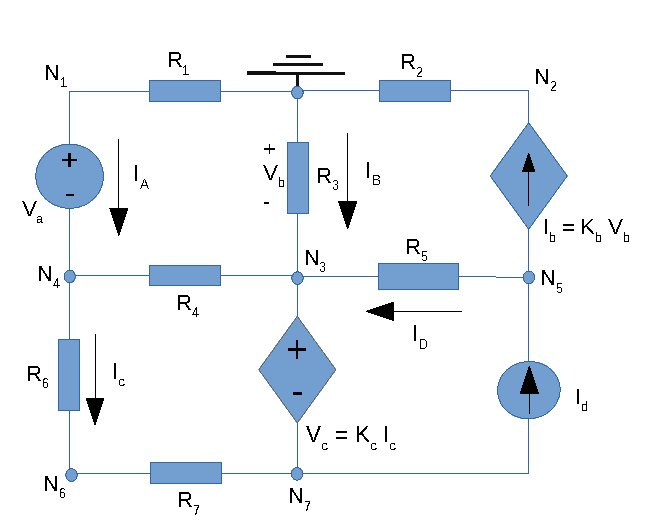
\includegraphics[width=0.6\linewidth]{circuito.pdf}
\caption{D Mesh with an additional voltage source} 
\label{fig:malhaD}
\end{figure}


\subsection{Operating Point Analysis for t$<$0}

The Table~\ref{tab:op1} shows the simulated operating point results for the circuit described in Figure~\ref{fig:circuito}, considering t$<$0, which means $V_{s}(t)$=$V_{s}$.

\begin{table}[!ht]
  \centering
  \begin{tabular}{|l|r|}
    \hline    
    {\bf Name} & {\bf Value [A or V]} \\ \hline
    \input{../sim/op1_tab}
  \end{tabular}
  \caption{Operating point. A variable preceded by @ is of type {\em current}
    and expressed in Ampere; other variables are of type {\it voltage} and expressed in
    Volt.}
  \label{tab:op1}
\end{table}

\subsection{Operating Point Analysis for t$=$0}

This second part covers the simulation of the circuit for t$=$0. To do that the capacitor is replaced with a voltage source $V_{x}$ = $V_{6}$ - $V_{8}$ using the values obtained in the previous section. This is necessary because for t$\leq$0 the voltage in the capacitor is the same. So to mantain the boundary conditions $V_{6}$ and $V_{8}$ the capacitor is replaced with the initial voltage source.
The results are presented on Table~\ref{tab:op2}.
\newline
\newline

\pagebreak
\begin{table}[!ht]
  \centering
  \begin{tabular}{|l|r|}
    \hline    
    {\bf Name} & {\bf Value [A or V]} \\ \hline
    \input{../sim/op2_tab}
  \end{tabular}
  \caption{Operating point. A variable preceded by @ is of type {\em current}
    and expressed in Ampere; other variables are of type {\it voltage} and expressed in
    Volt.}
  \label{tab:op2}
\end{table}


\subsection{Natural Solution}
In order to study the natural solution response of the circuit in the interval [0;20]ms using the boundary conditions ($V_{6}$ and $V_{8}$) calculated before, a transient analysis was realized. 
Fig.~\ref{fig:sim3} shows the plot of the required results.
\newline
\newline
\newline

\begin{figure}[H] \centering
\includegraphics[width=0.6\linewidth]{../sim/sim4.pdf}
\caption{Natural Response of $V_{6}$} 
\label{fig:sim3}
\end{figure}


\pagebreak

\subsection{Total Solution}

In the fourth section a total response of node 6 was perfomed, using the same procedure and interval of 3.3 with a initial sinusoidal voltage source $V_{s}(t)$ that has a frequency of 1000Hz. 
Fig.~\ref{fig:sim4} shows the plot of the required results.

\begin{figure}[H] \centering
\includegraphics[width=0.6\linewidth]{../sim/sim5.pdf}
\caption{Total Response of $V_{6}$ and $V_{s}$}
\label{fig:sim4}
\end{figure}




